% latex table generated in R 3.6.3 by xtable 1.8-4 package
% Thu Jan 18 11:47:23 2024
\begin{table}[ht]
\centering
\begin{tabular}{rlrrr}
  \hline
 & OTU & MeanRA & MedianRA & SE \\ 
  \hline
207340 & Roseomonas mucos & 0.00007201 & 0.00006850 & 0.00000427 \\ 
  441209 & Rhodobaca barguzinensi & 0.00005232 & 0.00005279 & 0.00000223 \\ 
  1591409 & Pseudohalocynthiibacter aestuariiviven & 0.00006593 & 0.00006454 & 0.00000280 \\ 
  1637862 & Burkholderia sp. LA-2-3-30-S1-D & 0.00006923 & 0.00006708 & 0.00000480 \\ 
  1267562 & Cupriavidus gilardii & 0.00006415 & 0.00004702 & 0.00001412 \\ 
  2771360 & Cupriavidus sp. ISTL & 0.00005041 & 0.00004090 & 0.00000934 \\ 
  859655 & Ralstonia solanacearum & 0.00003766 & 0.00003709 & 0.00000158 \\ 
  2724470 & Pseudomonas sp. BIGb042 & 0.00006858 & 0.00006637 & 0.00000388 \\ 
  1283291 & Pseudomonas sp. URMO17WK12:I1 & 0.00003928 & 0.00003849 & 0.00000178 \\ 
  384676 & Pseudomonas entomophila & 0.00007850 & 0.00008219 & 0.00000485 \\ 
  104087 & Pseudomonas frederiksbergensi & 0.00008436 & 0.00008030 & 0.00000470 \\ 
  1434072 & Halopseudomonas salegen & 0.00005233 & 0.00005134 & 0.00000488 \\ 
  69218 & Enterobacter cancerogenu & 0.00002917 & 0.00002789 & 0.00000138 \\ 
  1891675 & Pantoea alhag & 0.00001856 & 0.00001904 & 0.00000096 \\ 
  2033032 & Aeromonas sp. CA2 & 0.00003148 & 0.00003153 & 0.00000169 \\ 
  2622240 & Desulfopila & 0.00003303 & 0.00003349 & 0.00000208 \\ 
  67258 & Streptomyces cavourensi & 0.00007606 & 0.00007511 & 0.00000448 \\ 
  1929477 & Streptomyces solisilva & 0.00004807 & 0.00004541 & 0.00000312 \\ 
  145458 & Rathayibacter toxicu & 0.00004455 & 0.00004377 & 0.00000300 \\ 
  2714933 & Leucobacter coleopteroru & 0.00003709 & 0.00003446 & 0.00000282 \\ 
  85693 & Mycolicibacterium monacens & 0.00004709 & 0.00005015 & 0.00000206 \\ 
  38289 & Corynebacterium jeikeiu & 0.00006866 & 0.00006751 & 0.00000419 \\ 
  169292 & Corynebacterium aurimucosu & 0.00004290 & 0.00004373 & 0.00000250 \\ 
  43770 & Corynebacterium striatu & 0.00004517 & 0.00004610 & 0.00000165 \\ 
  39791 & Corynebacterium glucuronolyticu & 0.00004851 & 0.00004623 & 0.00000233 \\ 
  1683 & Bifidobacterium angulatu & 0.00003330 & 0.00003250 & 0.00000195 \\ 
  1603886 & Bifidobacterium lemuru & 0.00003561 & 0.00003560 & 0.00000143 \\ 
  1401 & Paenibacillus lautu & 0.00006885 & 0.00005823 & 0.00001235 \\ 
  714067 & Kroppenstedtia eburne & 0.00007132 & 0.00005045 & 0.00001543 \\ 
  1492710 & Oxynem & 0.00004465 & 0.00004352 & 0.00000238 \\ 
  938406 & Calothrix brevissim & 0.00001466 & 0.00001402 & 0.00000224 \\ 
  109266 & Anabaenopsis circulari & 0.00000808 & 0.00000784 & 0.00000116 \\ 
  56956 & Thermus brockianu & 0.00004538 & 0.00004655 & 0.00000234 \\ 
  2527976 & Gimesia fumarol & 0.00004065 & 0.00004030 & 0.00000231 \\ 
  2528019 & Planctopirus ephydatia & 0.00005018 & 0.00004821 & 0.00000336 \\ 
  1679444 & Akkermansia glycaniphil & 0.00005856 & 0.00005763 & 0.00000201 \\ 
  665571 & Spirochaeta thermophila & 0.00003158 & 0.00003442 & 0.00000174 \\ 
  1441386 & Athalassotoga saccharophil & 0.00001002 & 0.00000754 & 0.00000240 \\ 
  660522 & Haloplanus aerogene & 0.00007728 & 0.00007392 & 0.00000381 \\ 
  2257 & Natronomonas pharaoni & 0.00003864 & 0.00003487 & 0.00000190 \\ 
  588898 & Natronorubrum daqingens & 0.00004382 & 0.00004437 & 0.00000224 \\ 
  536044 & Methanolobus zinder & 0.00000337 & 0.00000355 & 0.00000032 \\ 
  92945 & Ketogulonicigenium vulgar & 0.00006901 & 0.00008197 & 0.00001043 \\ 
   \hline
\end{tabular}
\caption{Keystone OTUs of } 
\end{table}
\begin{figure}
\centering
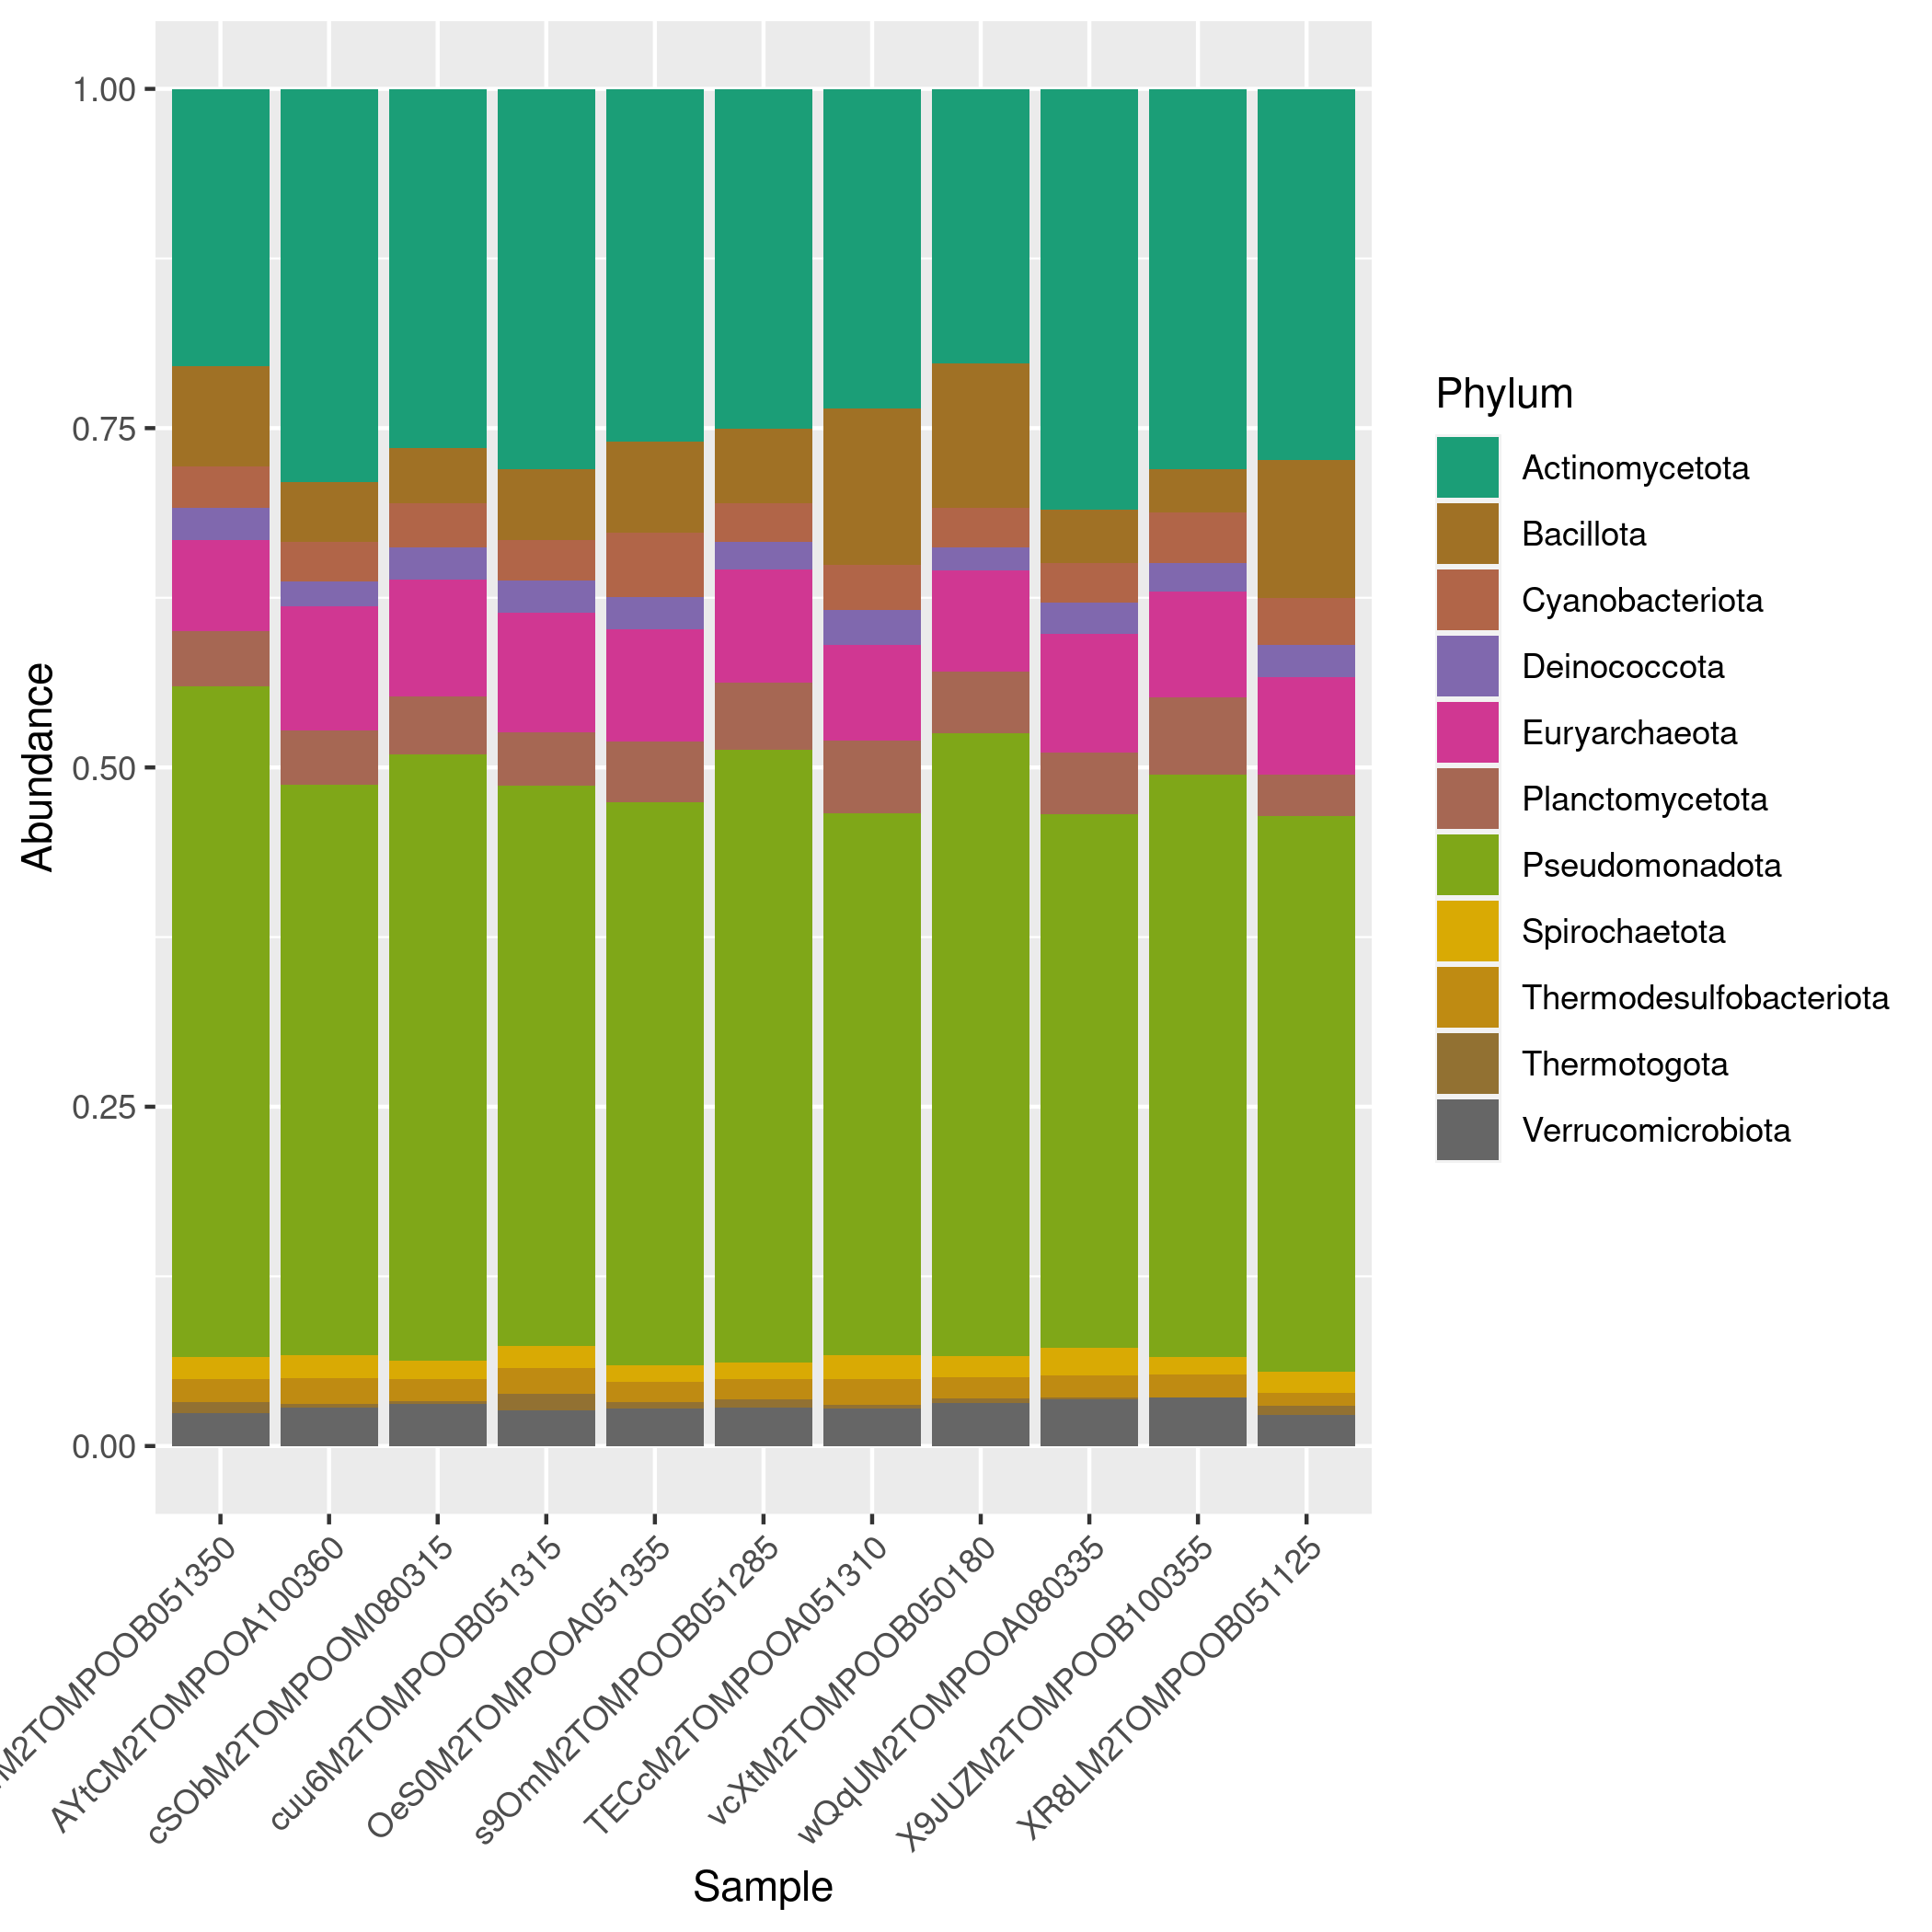
\includegraphics[scale = 0.8]{tomate_aleatorio1_4.csv_relative_abundance_Phylum.png}
\caption{Relative abundance by phyla of keystone OTUs }
\label{fig:tomate_aleatorio1_4.csv_phyla}
\end{figure}
\begin{figure}
\centering
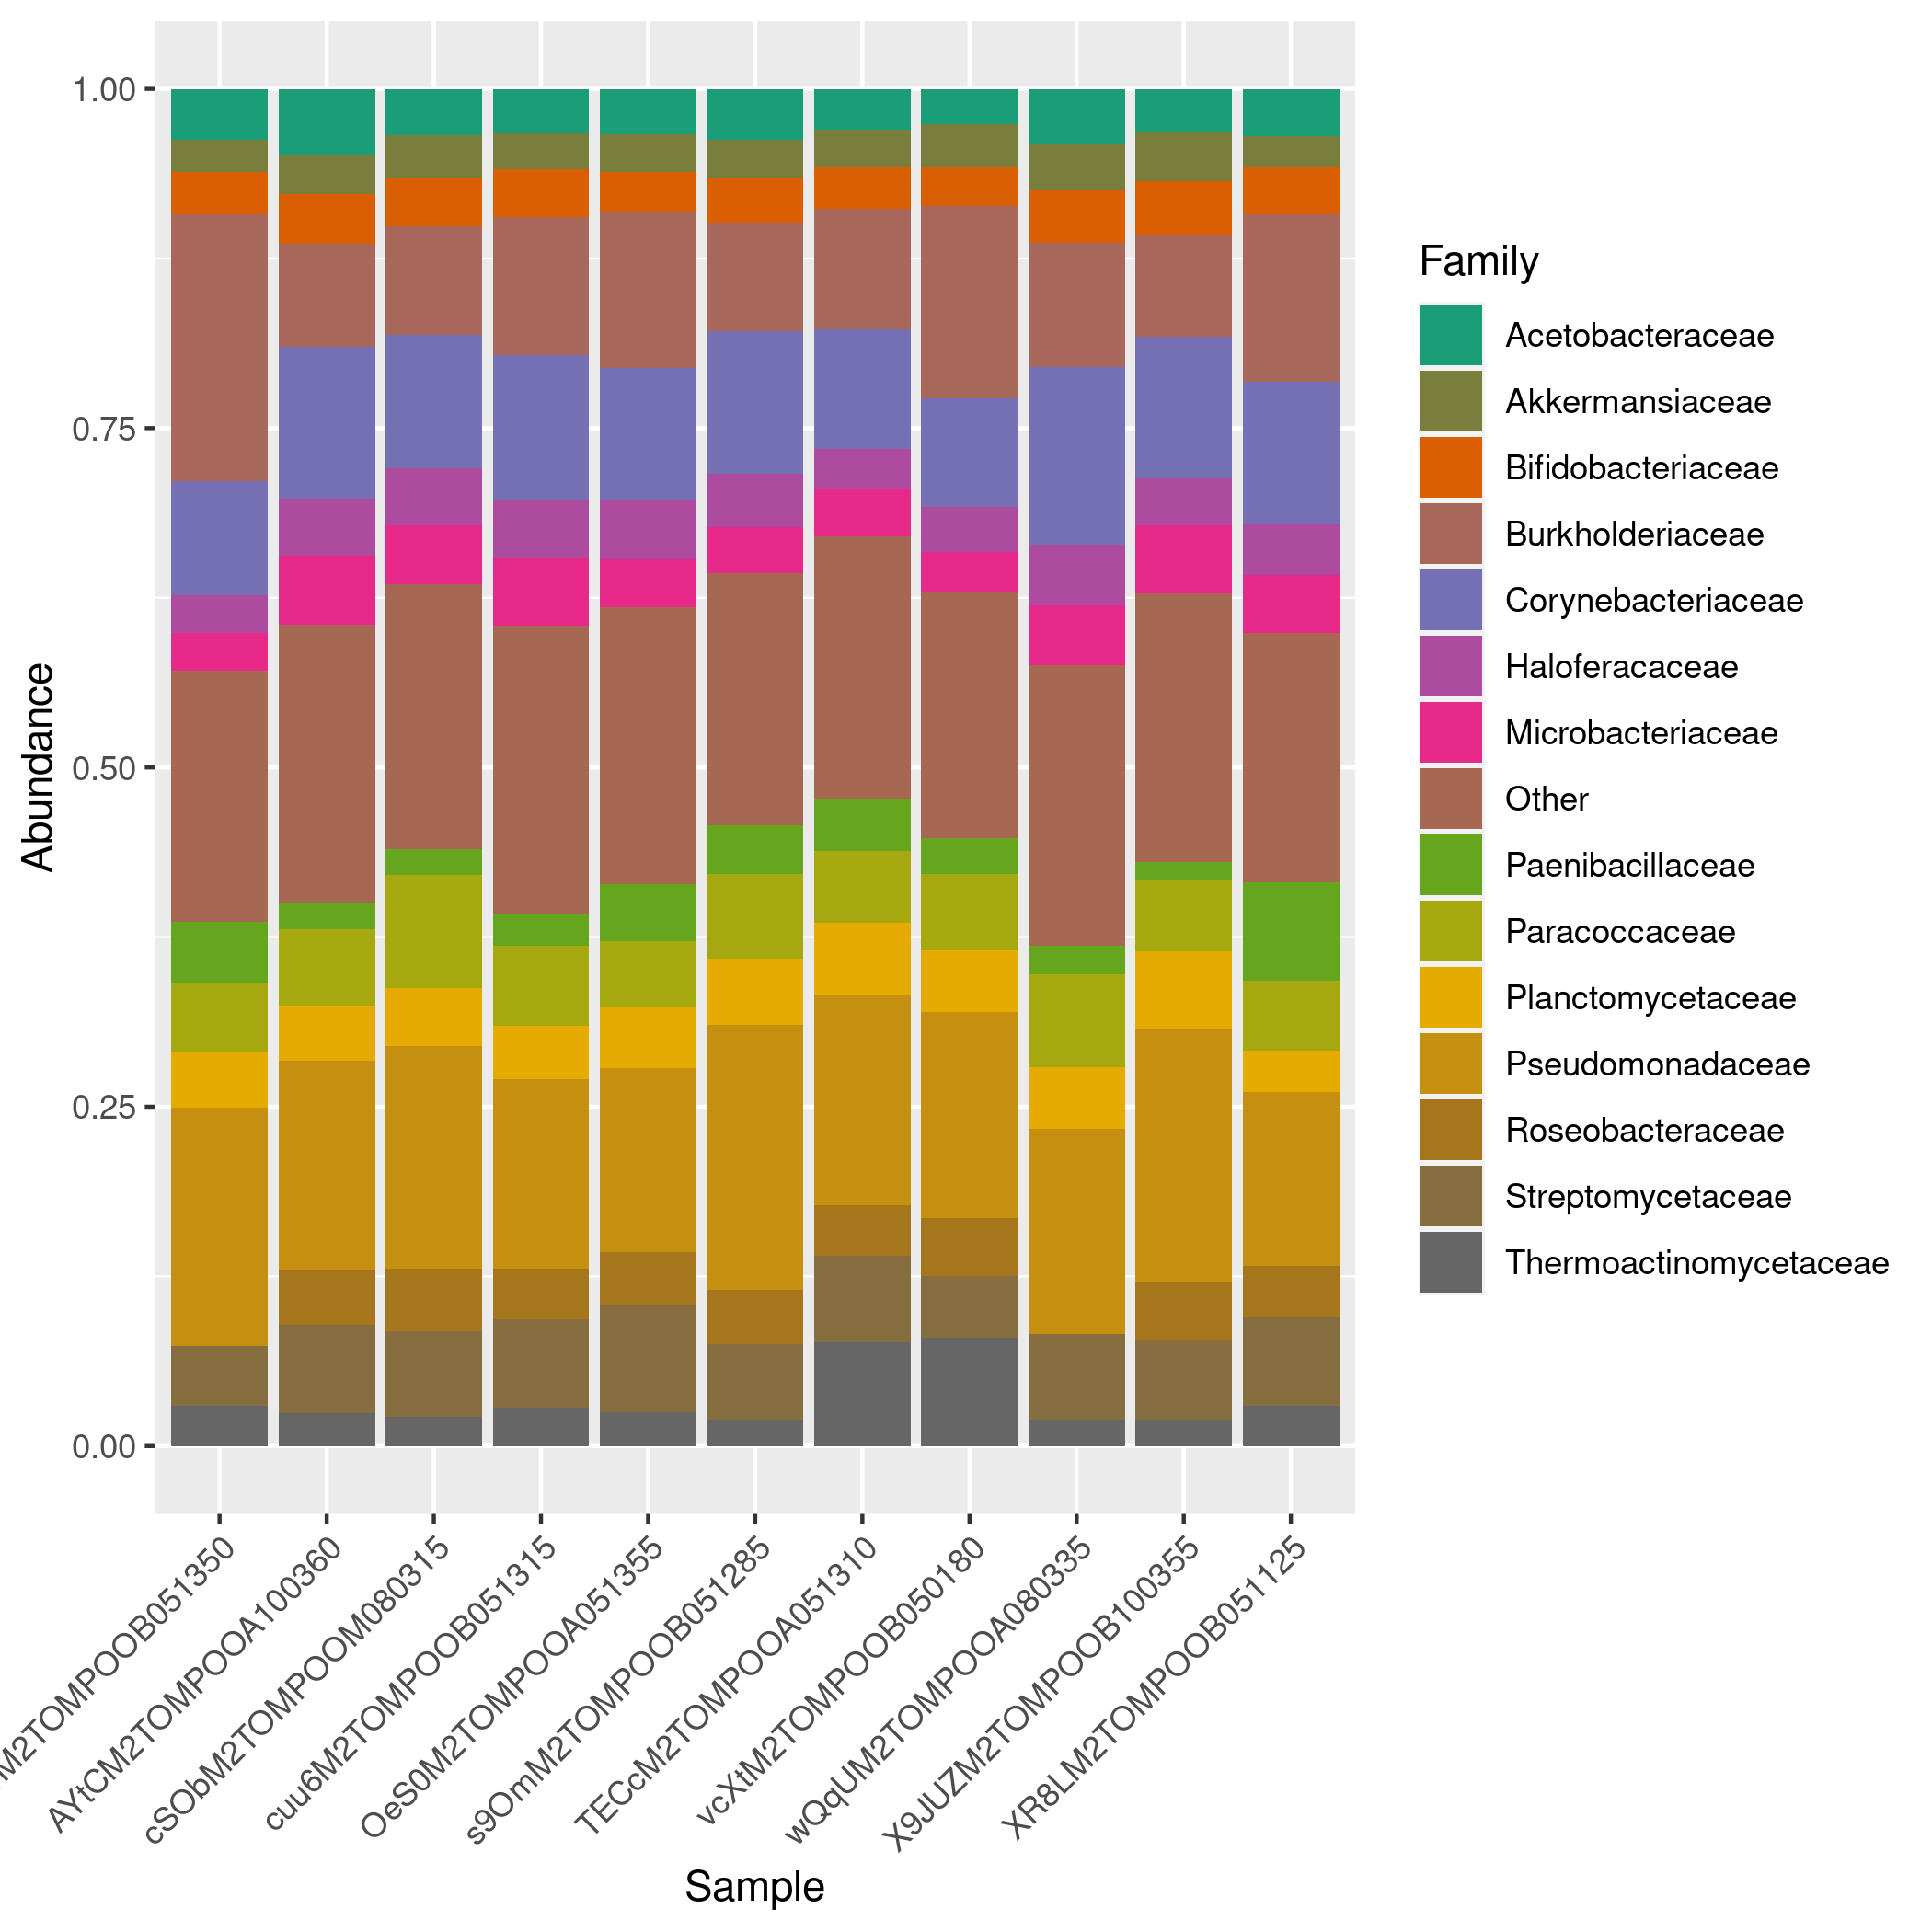
\includegraphics[scale = 0.8]{tomate_aleatorio1_4.csv_relative_abundance_Family.png}
\caption{Relative abundance by families of keystone OTUs }
\label{fig:tomate_aleatorio1_4.csv_family}
\end{figure}
\begin{figure}
\centering
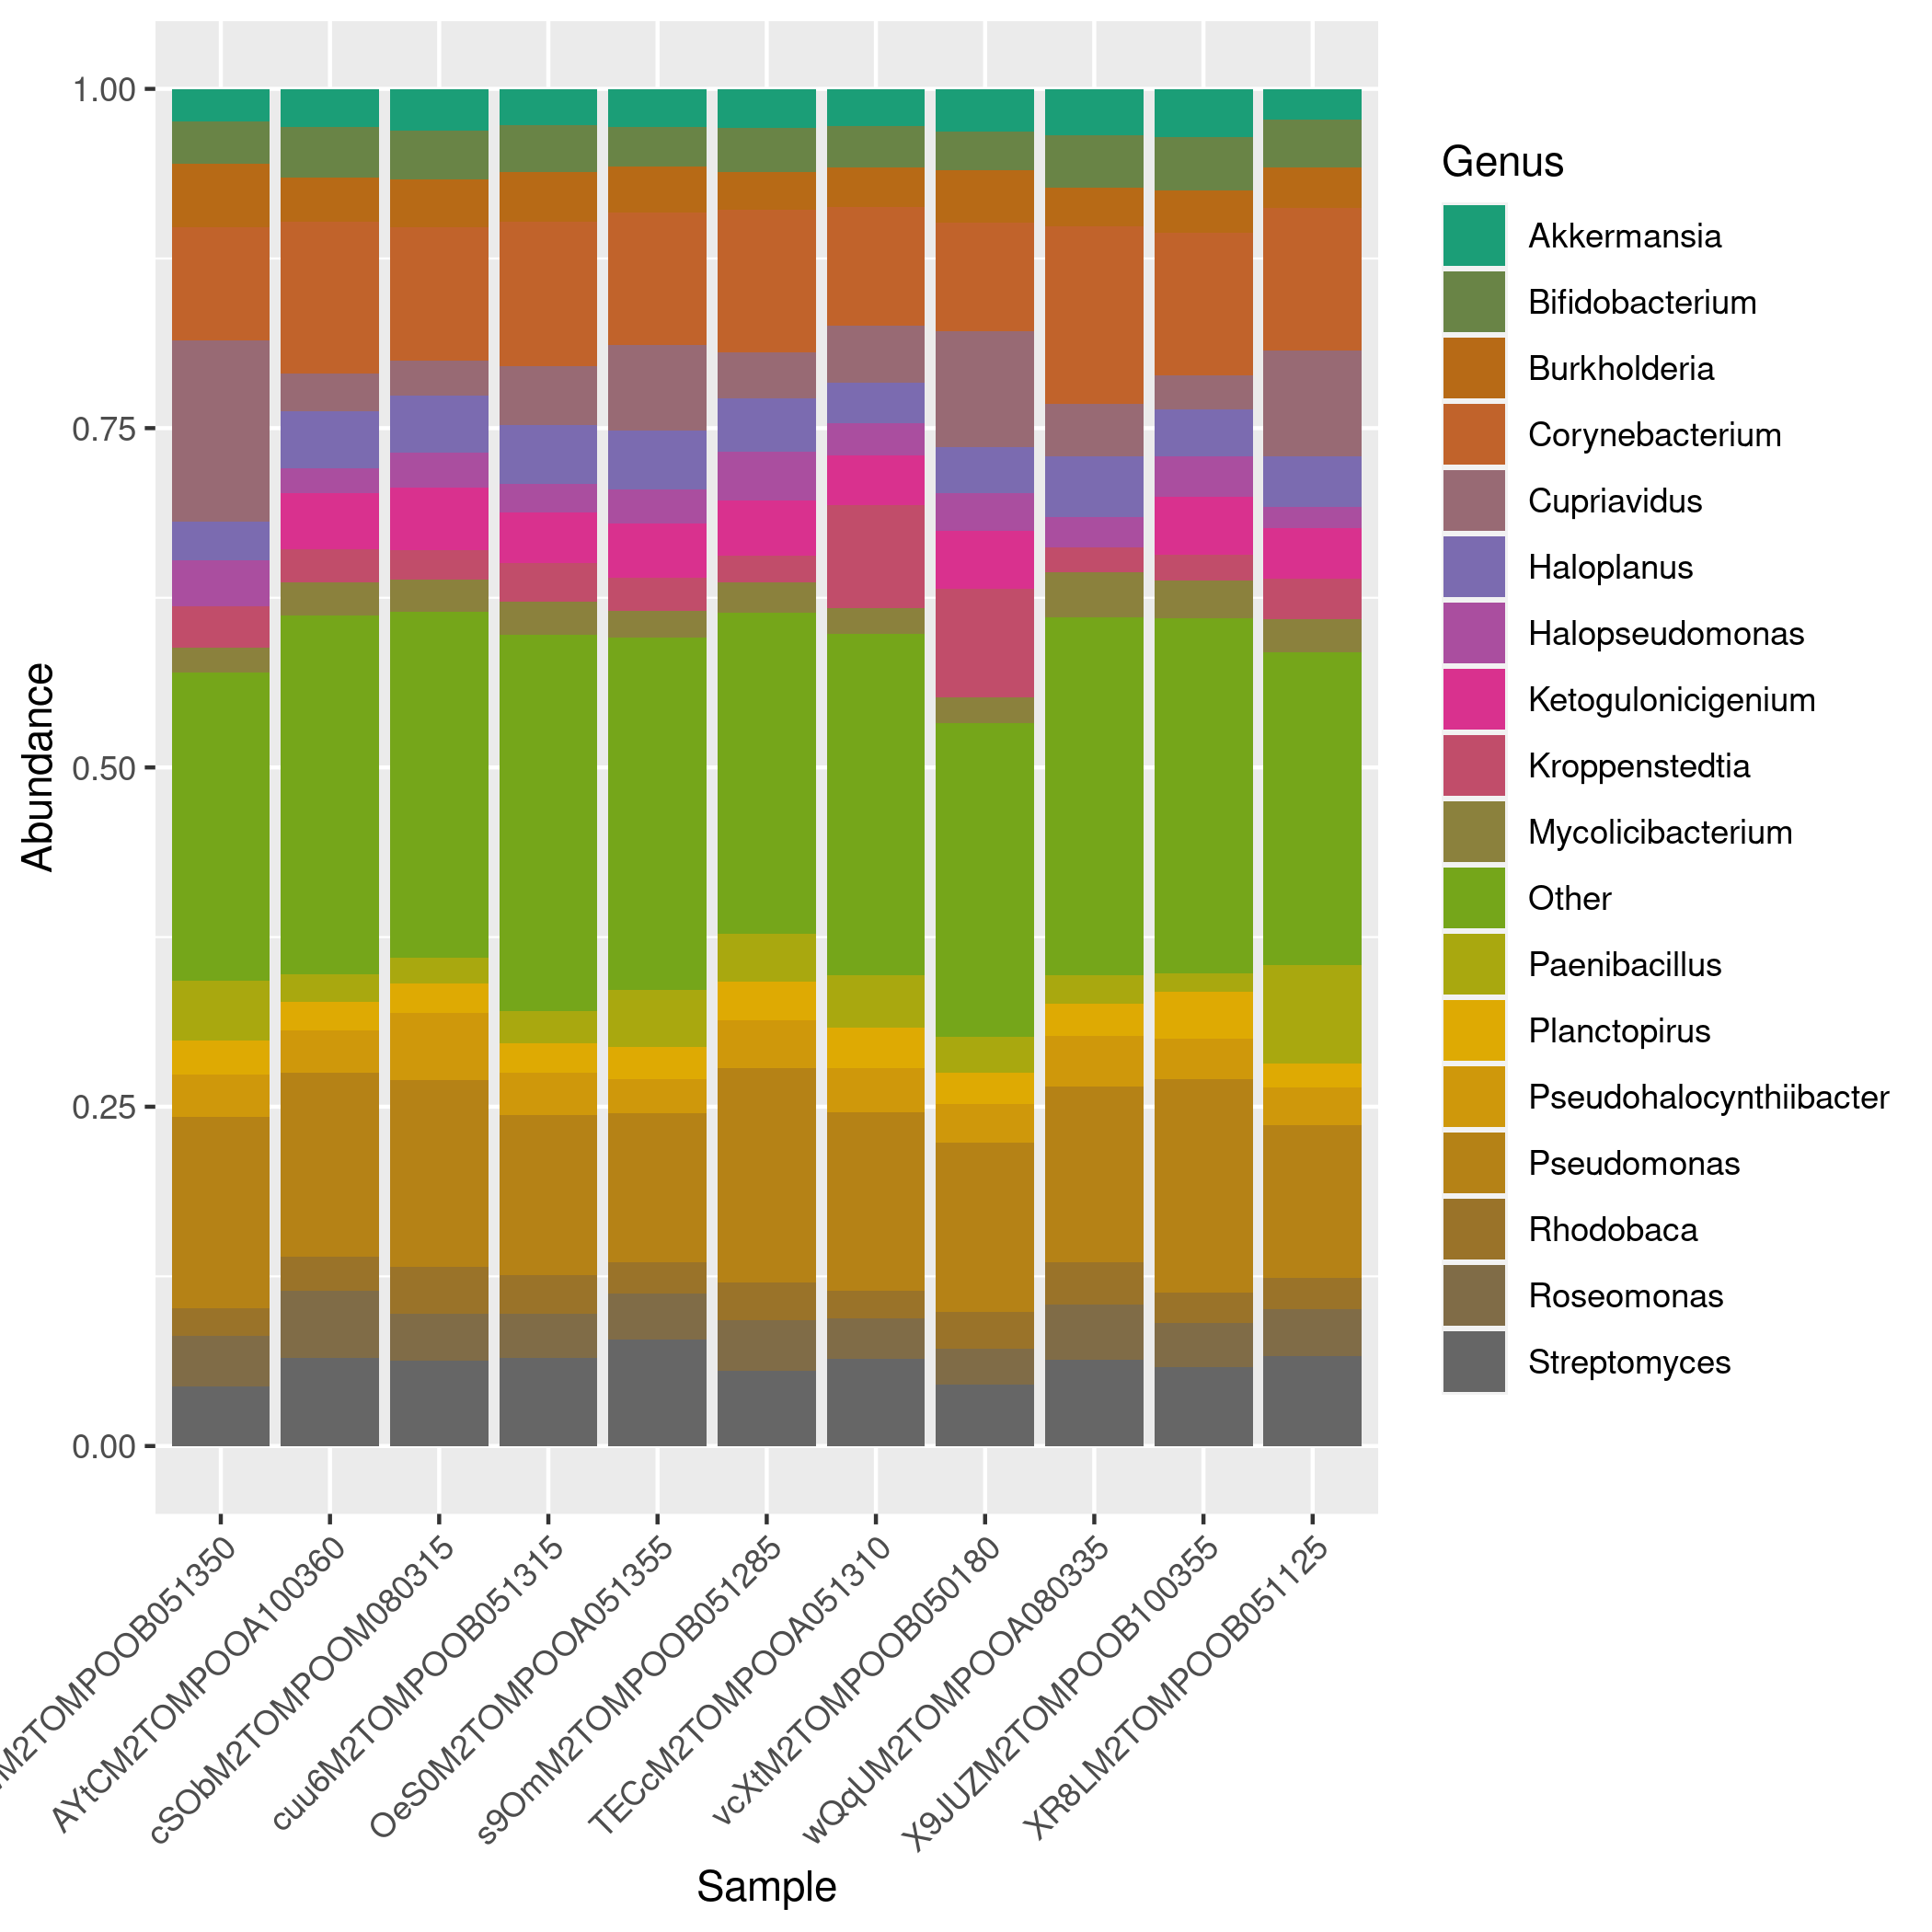
\includegraphics[scale = 0.8]{tomate_aleatorio1_4.csv_relative_abundance_Genus.png}
\caption{Relative abundance by genera of keystone OTUs }
\label{fig:tomate_aleatorio1_4.csv_genus}
\end{figure}
\begin{figure}
   \centering
   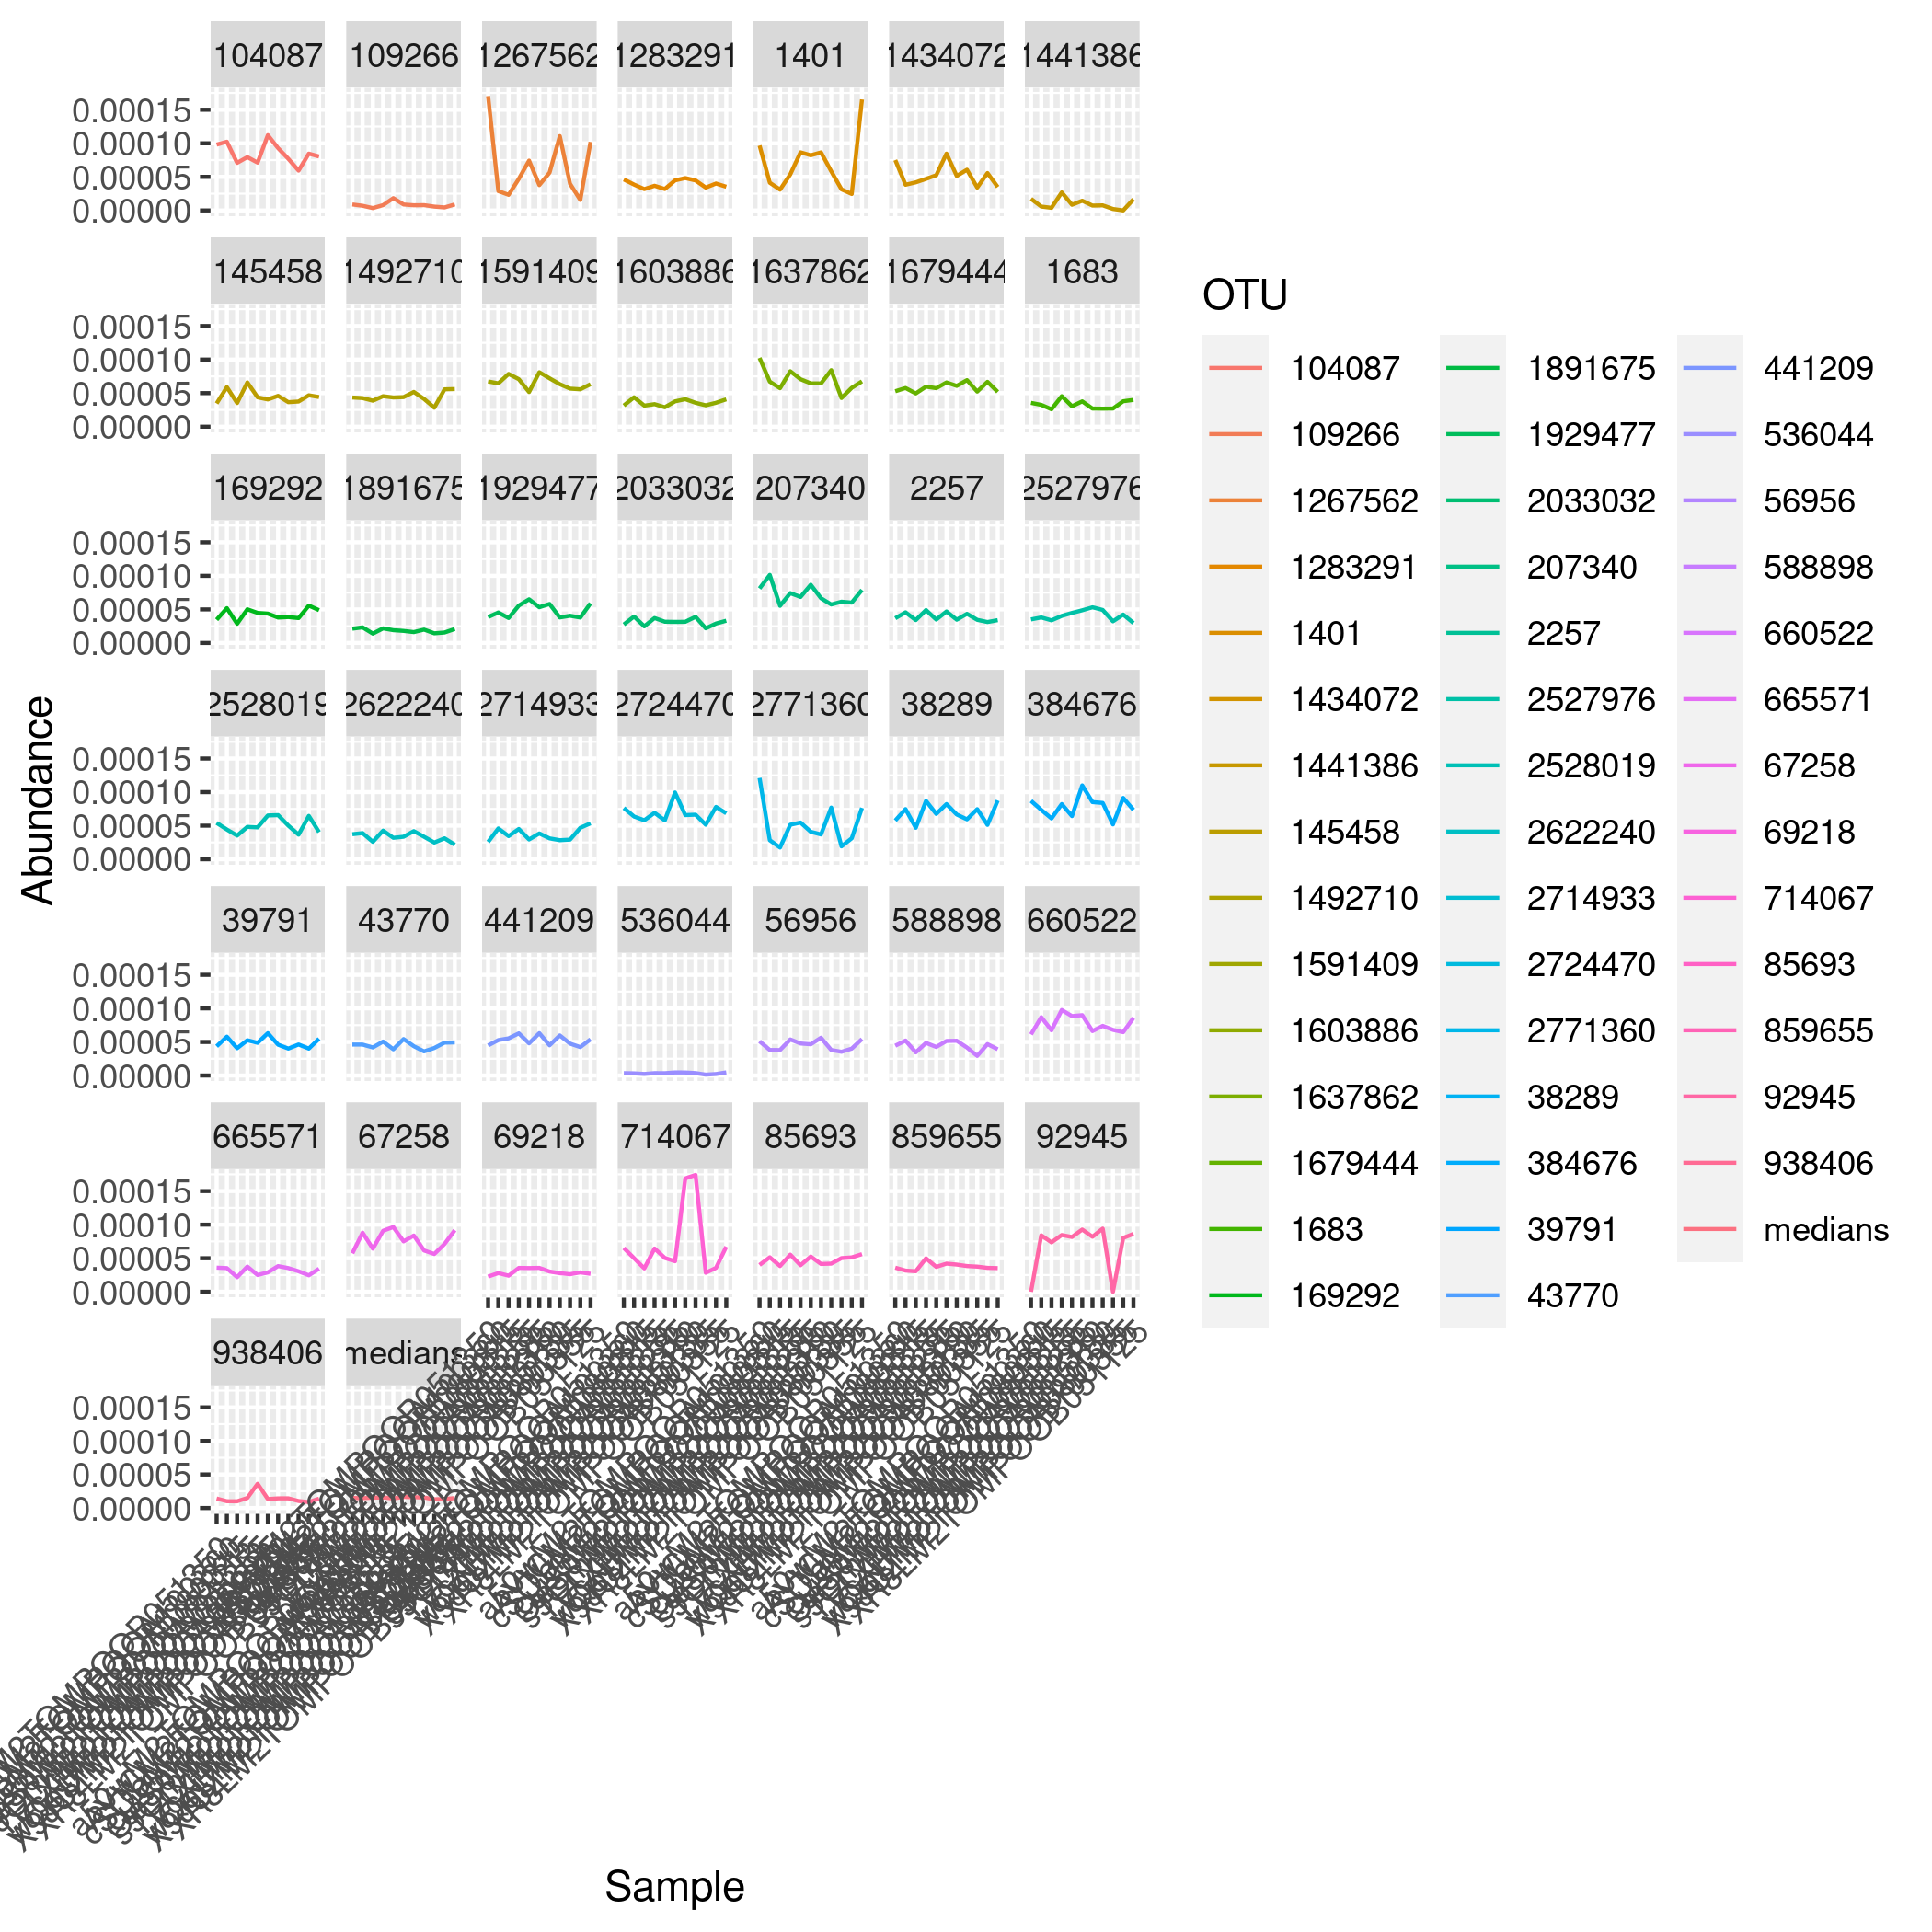
\includegraphics[scale = 0.8]{abundance_tomate_aleatorio1_4.csv_key_otus_medians.png}
   \caption{Plots representing relative abundance of each keystone OTU and one representing the median relative abundance  across samples of rhizosphere of tomate_aleatorio1_4.csv. Most keystone OTUs have relative abundance bigger than the median across all samples.  }
   \label{key_otus_vs_medians_tomate_aleatorio1_4.csv}
\end{figure}
\begin{figure}
 \centering
 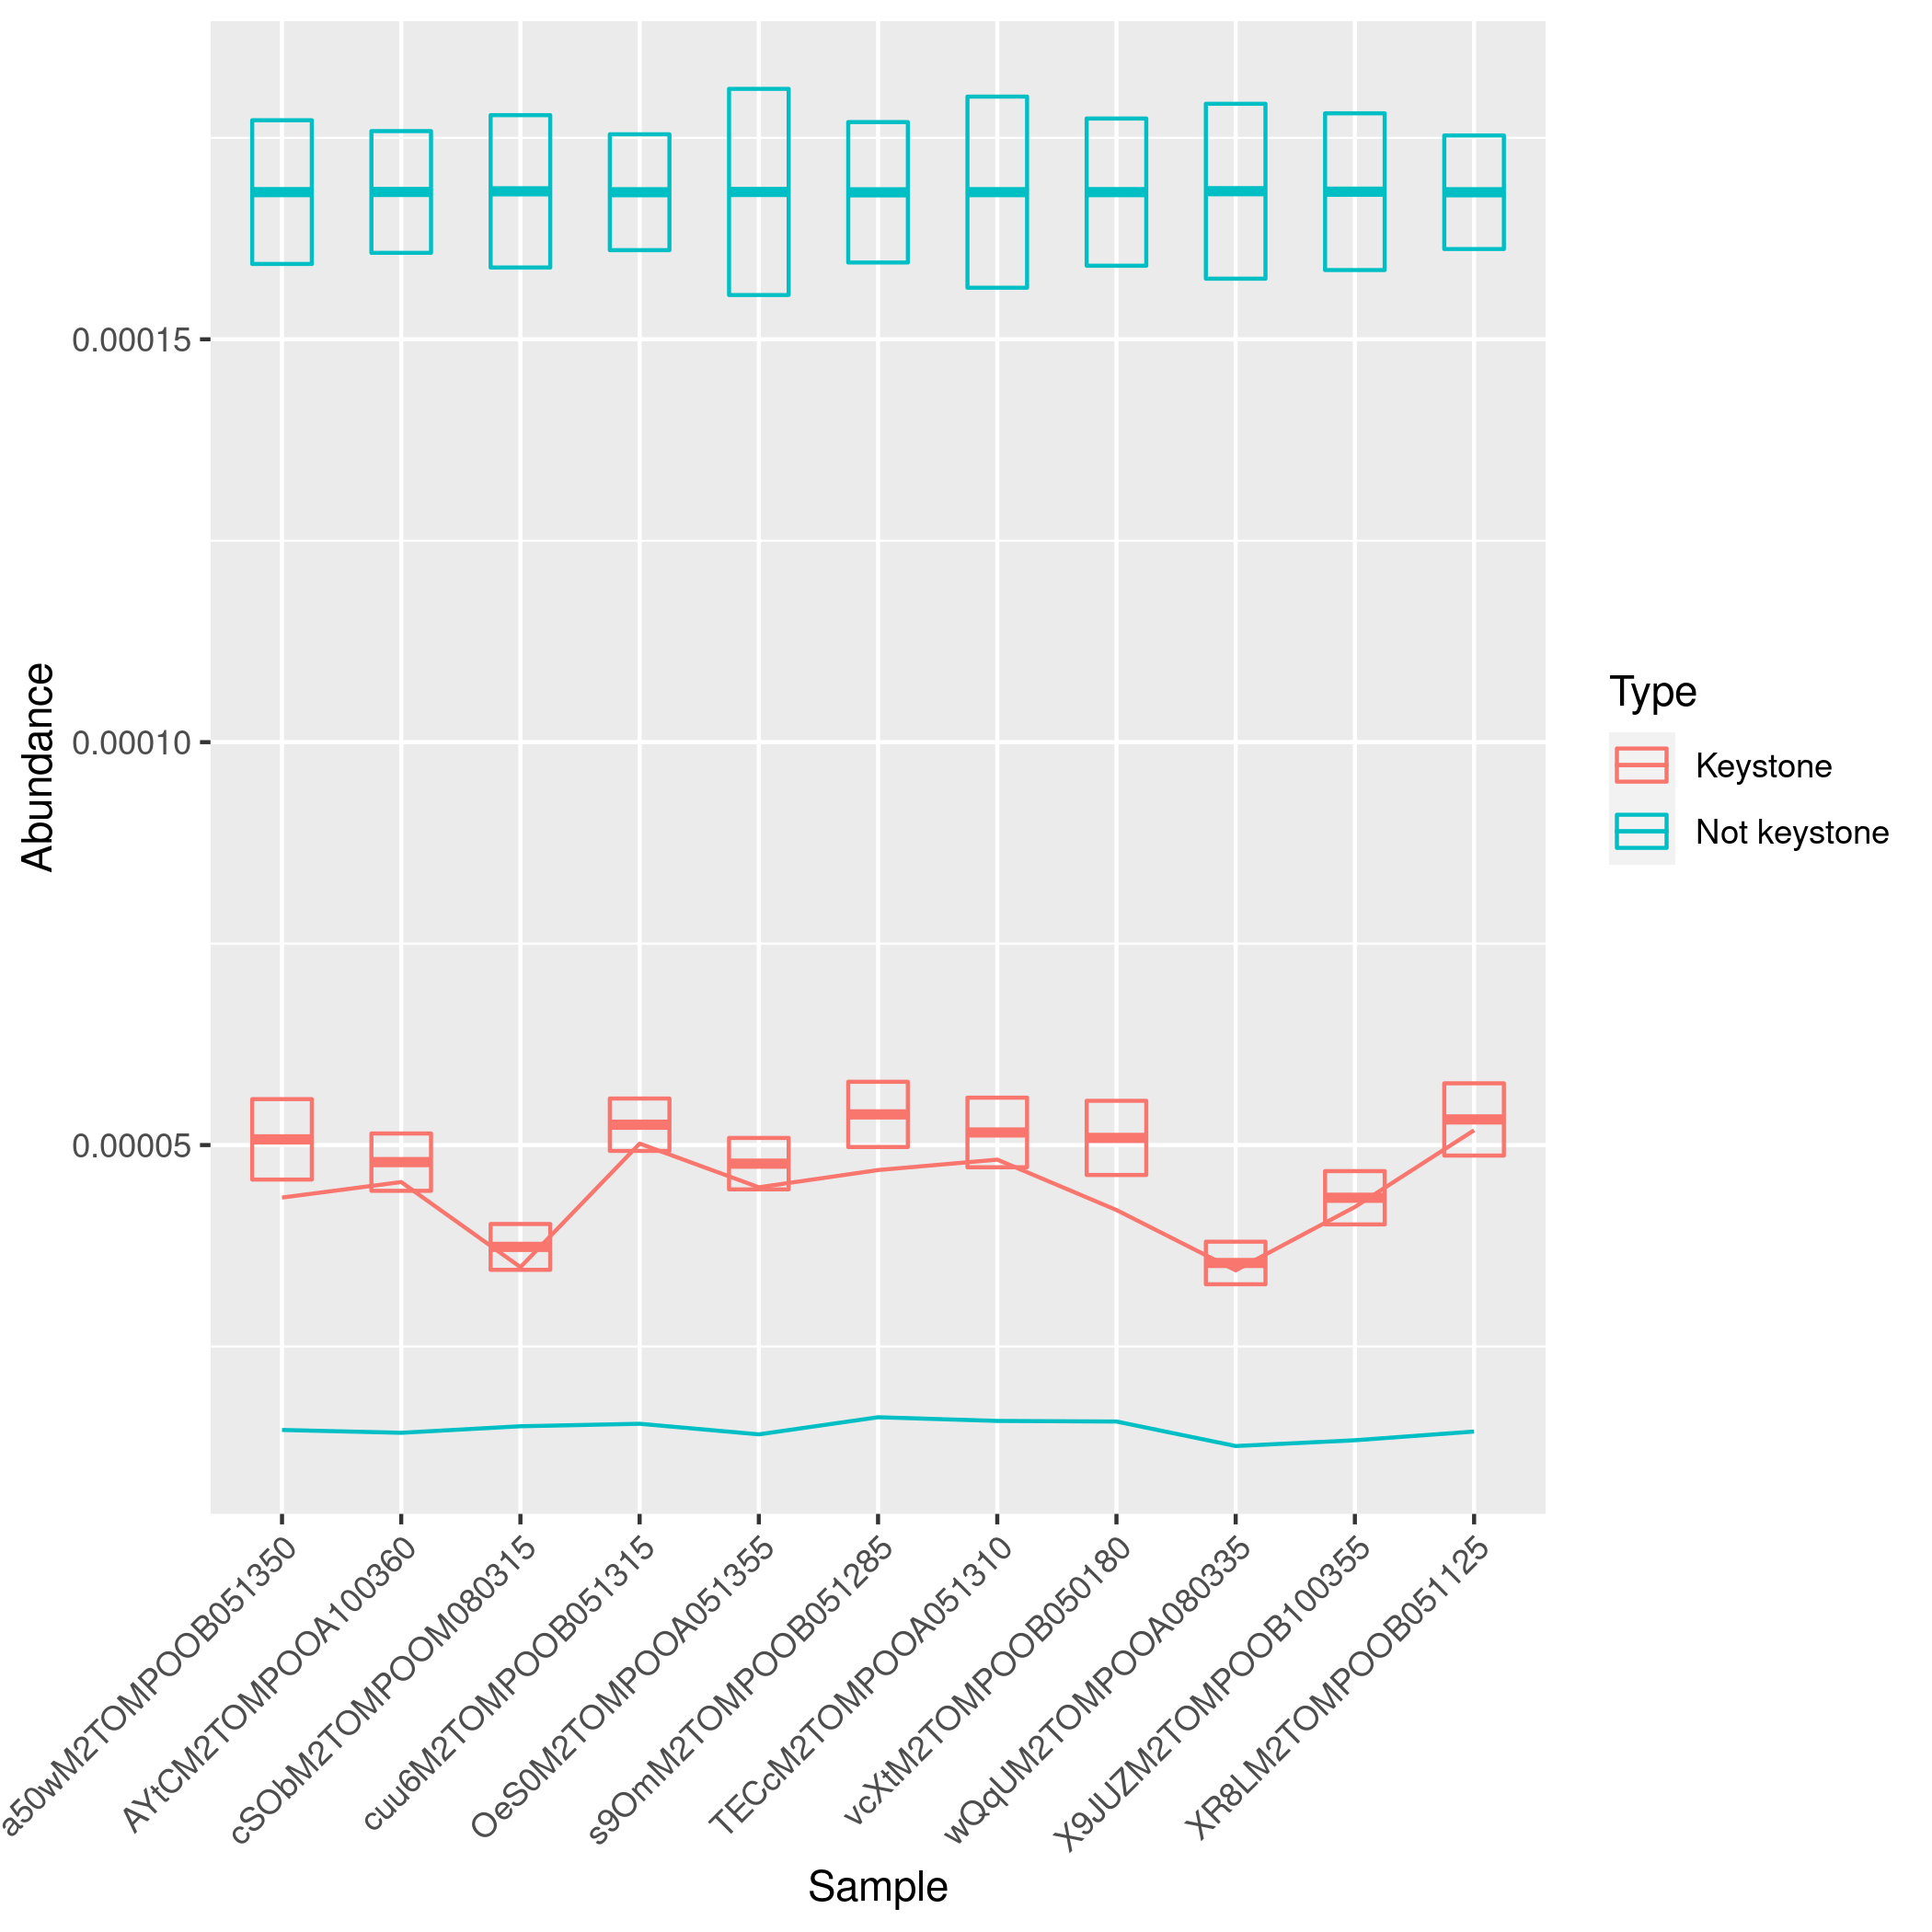
\includegraphics[scale = 0.75]{mean_median_key_vs_not_key_tomate_aleatorio1_4.csv.png}
\caption{Boxes represent mean and standard error in the distribution of corresponding samples. Lines represent the corresponding medians. In these samples of rhizosphere oftomate_aleatorio1_4.csv}
\label{mean_median_tomate_aleatorio1_4.csv}
\end{figure}
\begin{figure}
   \centering
   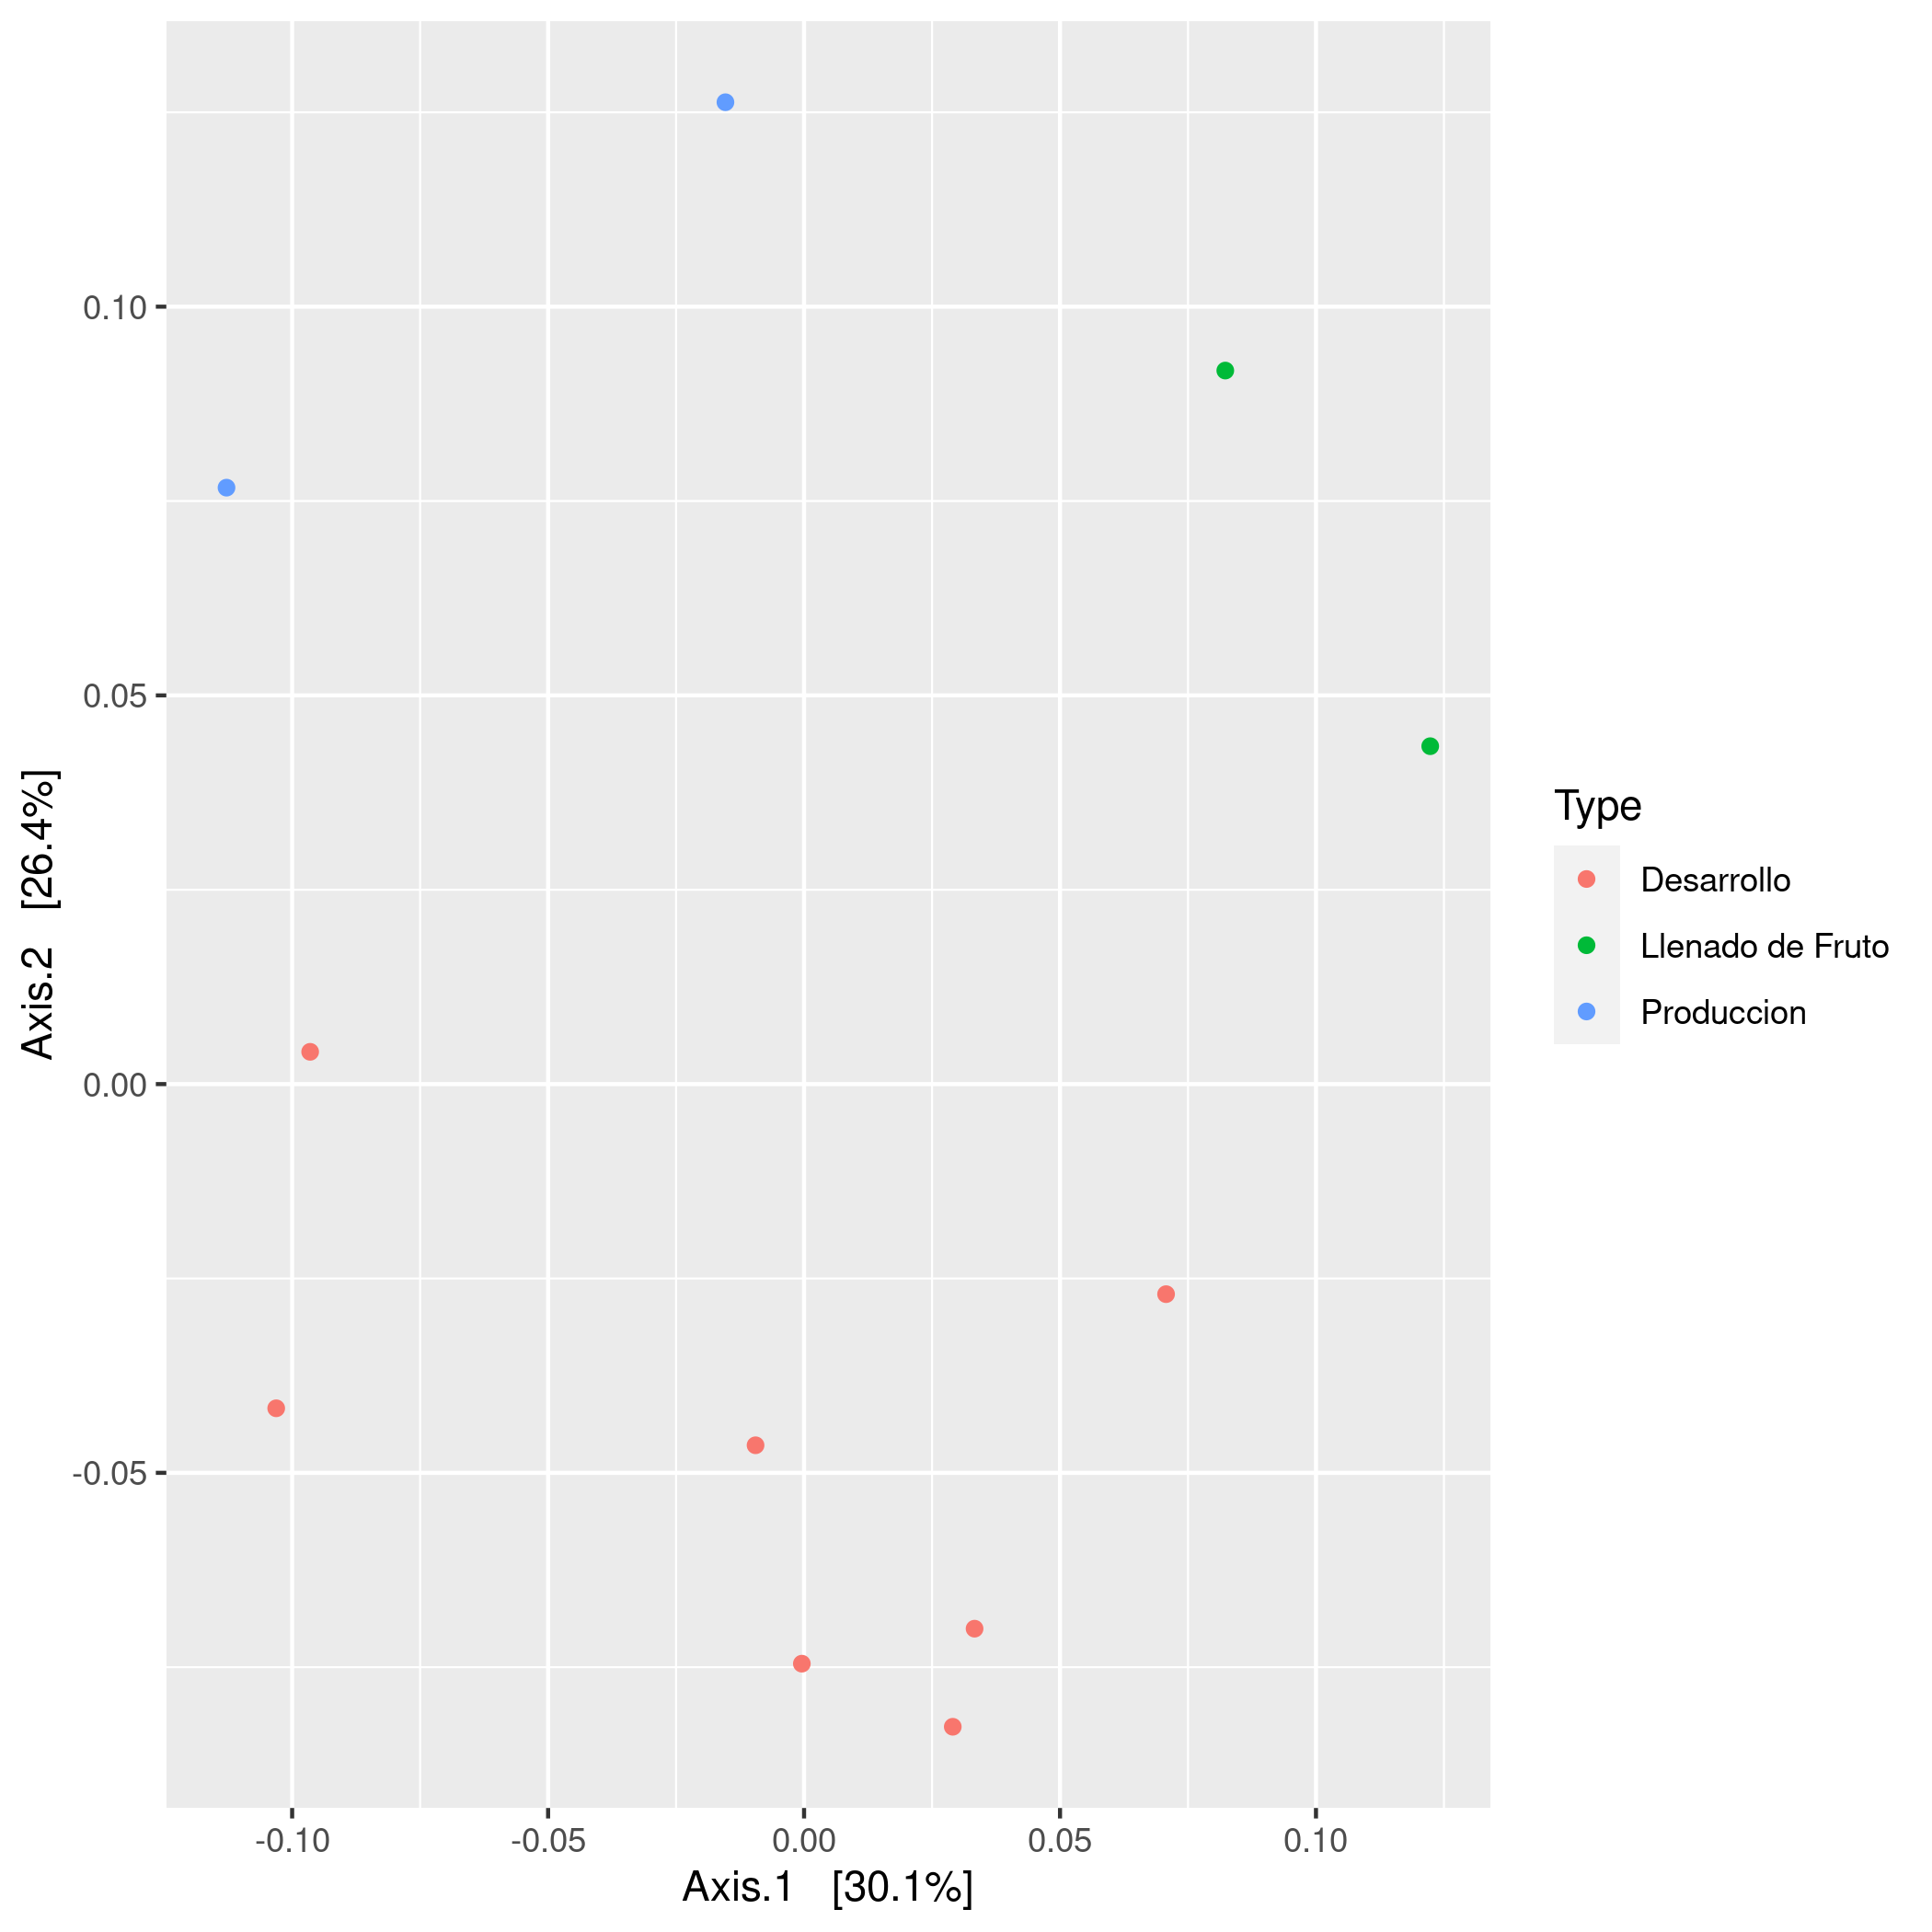
\includegraphics[scale = 0.7]{pcoa_muestras_tomate_aleatorio1_4.csv.png}
 \caption{PCoA analysis with Bray-Curtis distance of rhizosphere samples of tomate_aleatorio1_4.csv.}
 \label{fig:tomate_aleatorio1_4.csv_pcoa}
\end{figure}
\begin{figure}
  \centering
  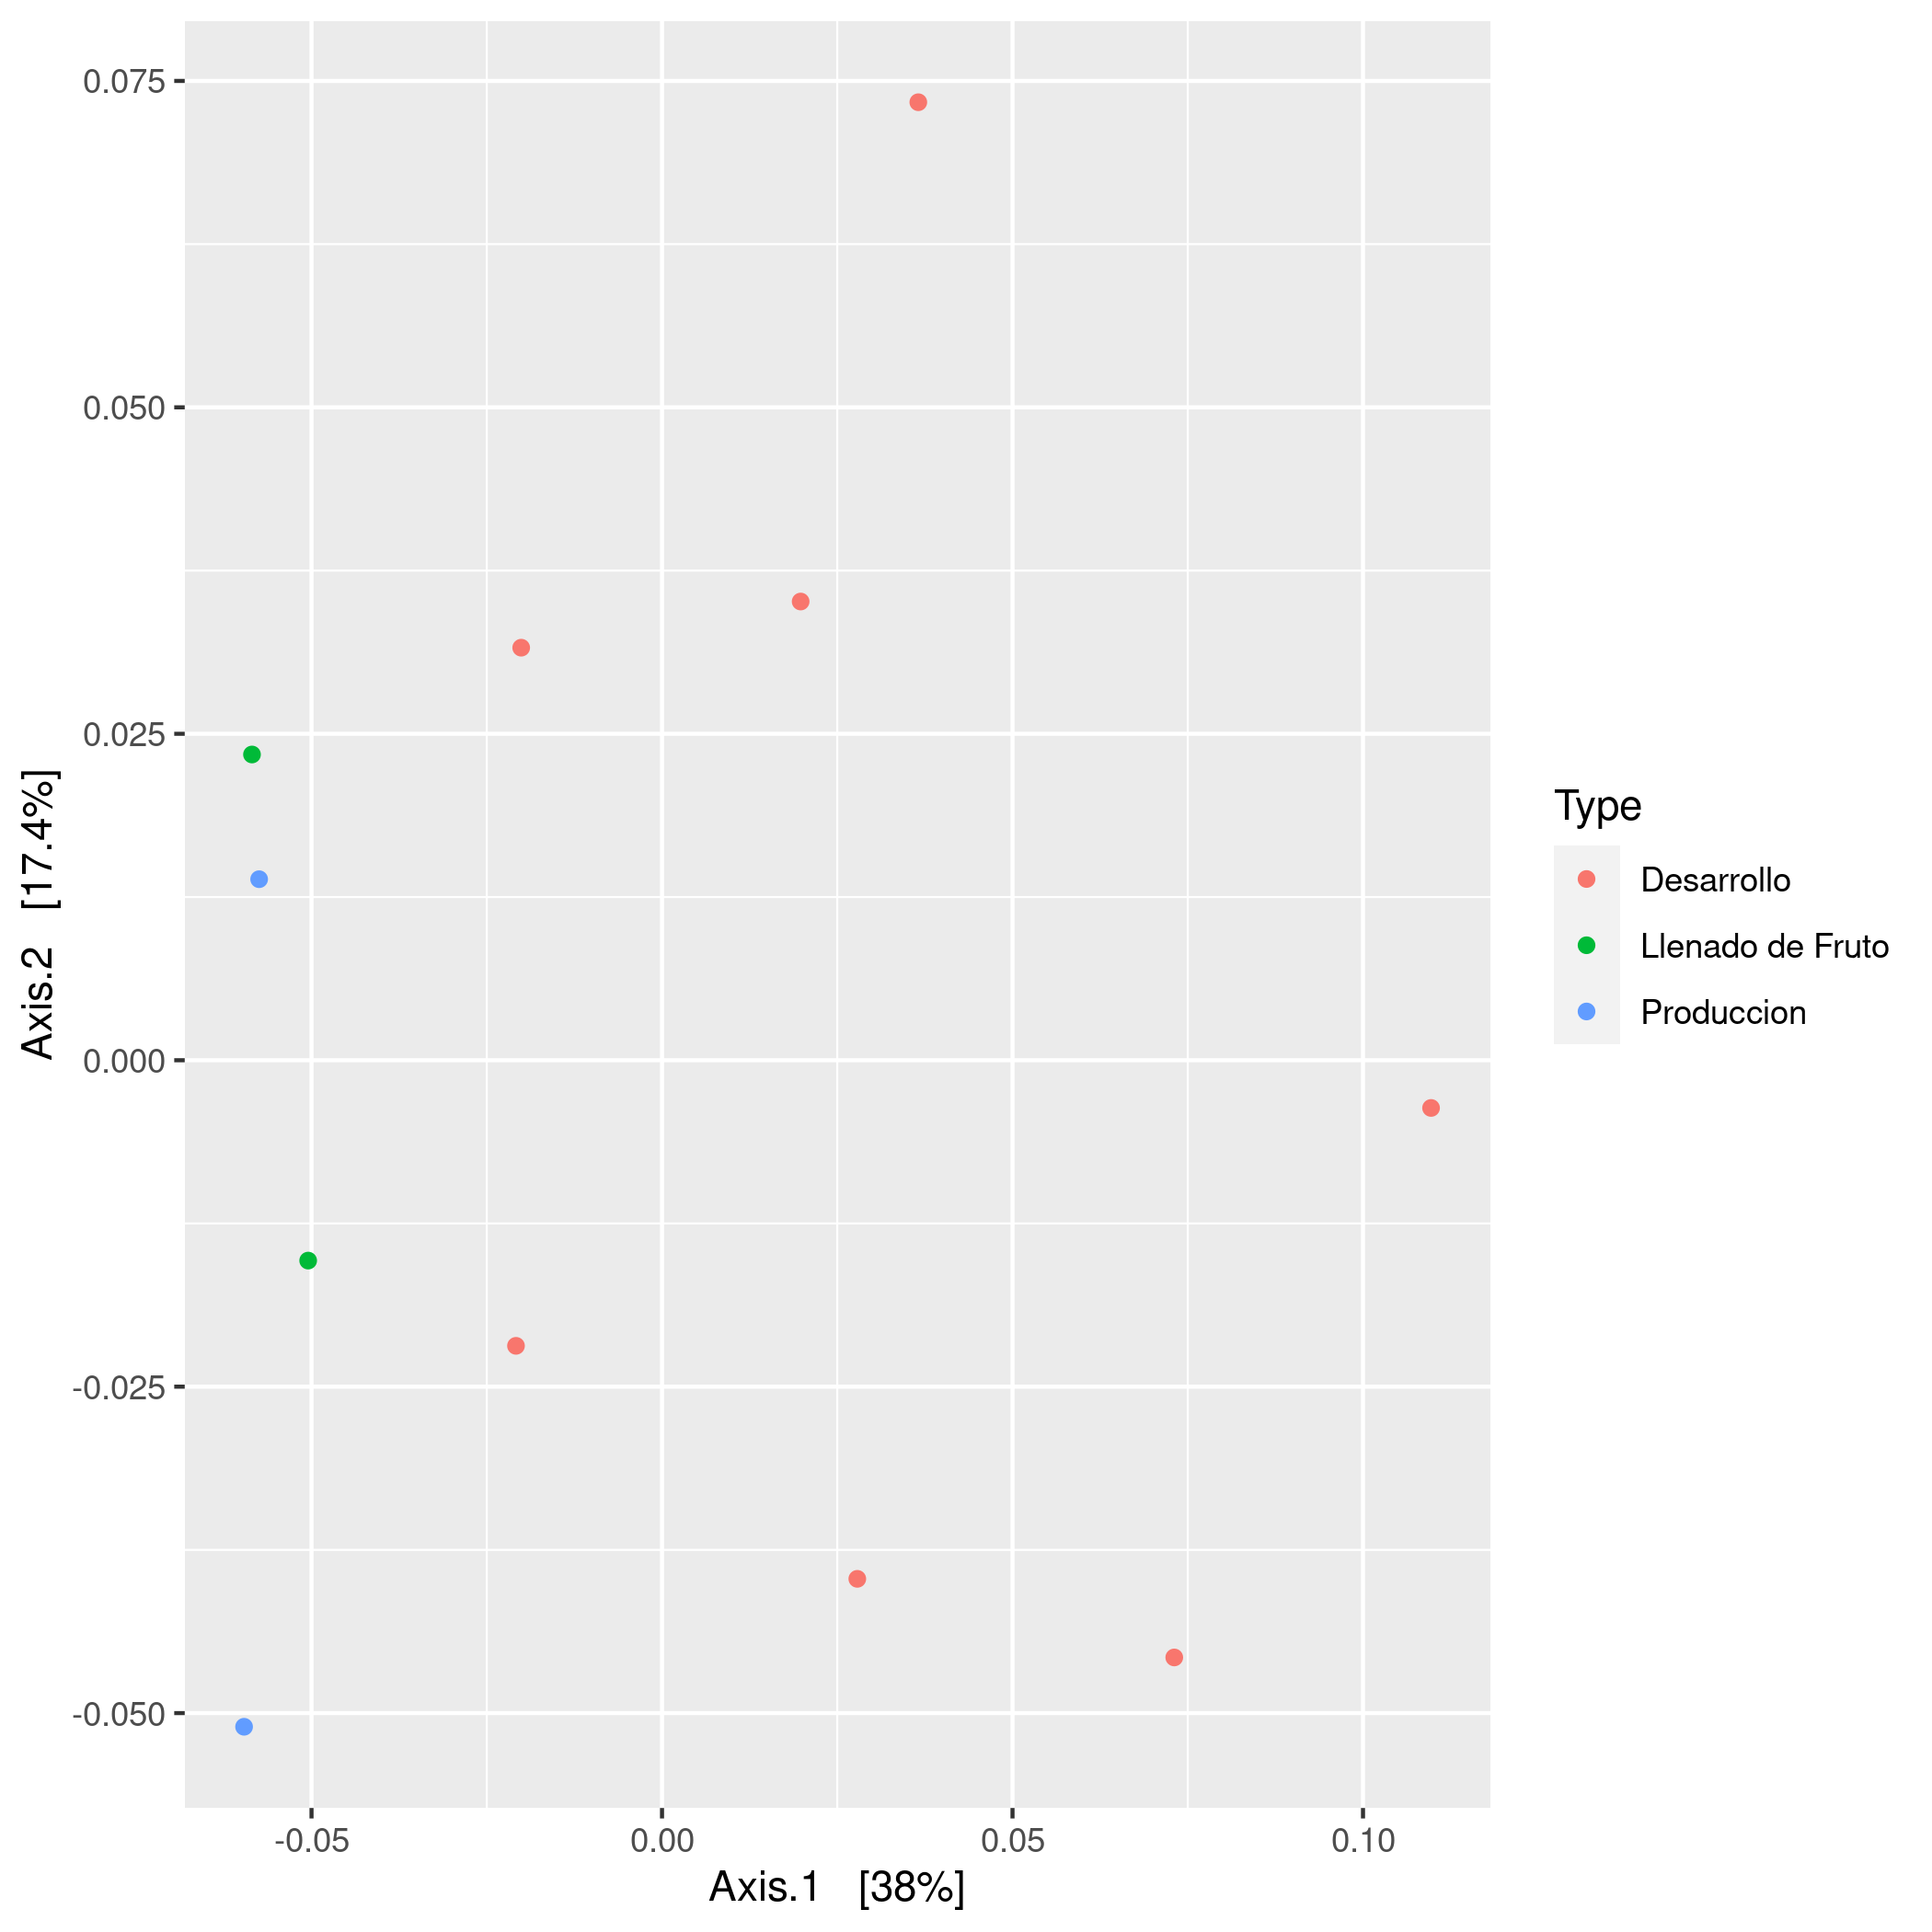
\includegraphics[scale = 0.7]{pcoa_key_otus_tomate_aleatorio1_4.csv.png}
  \caption{PCoA analysis with Bray-Curtis distance of rhizosphere samples of tomate_aleatorio1_4.csv, restricted to keystone OTUs.}
  \label{fig:tomate_aleatorio1_4.csv_pcoa_key_otus}
\end{figure}
